\documentclass[11pt,a4paper]{book}
\usepackage[top=2.5cm,bottom=2.5cm,left=2.5cm,right=2.5cm,headsep=10pt,letterpaper]{geometry}
\usepackage{physics}
\usepackage{siunitx}
\usepackage{graphicx}
\usepackage{amsmath}
\usepackage{amssymb}
\usepackage{amsthm}
\usepackage{thmtools}
\usepackage{tikz}
\usepackage{hyperref}
\usepackage{cleveref} % cleverref must come AFTER hyperref
\usepackage{bm}
\usepackage{xcolor}
\usepackage[font=small]{caption}
\usepackage[euler]{textgreek}
\usepackage[perpage]{footmisc}
\usepackage{pythonhighlight}

\usepackage[shortlabels]{enumitem}
\setlist[itemize]{noitemsep}
\setlist[enumerate]{noitemsep}

\setlength{\parindent}{1em}
\setlength{\parskip}{0.5em}
\setlength{\footnotesep}{1em}

% https://tex.stackexchange.com/questions/300340/topsep-itemsep-partopsep-and-parsep-what-does-each-of-them-mean-and-wha
\setlist[itemize]{noitemsep, topsep=-\parskip, parsep=0pt}
\setlist[enumerate]{noitemsep, topsep=-\parskip, parsep=0pt}

\renewcommand{\baselinestretch}{1.1}
\renewcommand{\thefootnote}{\fnsymbol{footnote}}

% below from https://tex.stackexchange.com/questions/80286/can-i-define-a-new-unit-that-behaves-like-ang-in-siunitx
\newcommand*{\hms}[2][]{{
    \ang[
        math-degree=\textsuperscript{h},             % Solution 2
        text-degree=\textsuperscript{h},             % Solution 2
        math-arcminute=\textsuperscript{m},          % Solution 2
        text-arcminute=\textsuperscript{m},          % Solution 2
        math-arcsecond=\textsuperscript{s},          % Solution 2
        text-arcsecond=\textsuperscript{s},          % Solution 2
        #1]{#2}%
}}

\newcommand*{\m}[2][]{{
    \ang[
        math-degree=\textsuperscript{m},             % Solution 2
        text-degree=\textsuperscript{m},             % Solution 2
        #1]{#2}%
}}

\renewcommand{\lg}{\ensuremath{\log_{10}}}
\newcommand{\degr}{\ensuremath{\degree}}
\newcommand{\sun}{\ensuremath{\odot}}
\newcommand{\earth}{\ensuremath{\oplus}}

\newcommand{\lineseg}[1]{\ensuremath{\overline{\mathrm{#1}}}}
\newcommand{\triang}[1]{\ensuremath{\triangle \mathrm{#1}}}
\newcommand{\rect}[1]{\ensuremath{\Box \mathrm{#1}}}
\newcommand{\linevec}[1]{\ensuremath{\overrightarrow{\mathrm{#1}}}}


\newcommand{\sep}{\quad;\quad}


\declaretheorem[
  thmbox={style=M, bodystyle=\normalfont\small, headstyle=\small\color{red!55!black}\bfseries Ex \upshape\theex}
  ]{ex}
\declaretheorem[
  thmbox={style=M, bodystyle=\normalfont\small, headstyle=\small\color{blue!55!black}\bfseries Thm \upshape\thethm}
  ]{thm}
\declaretheorem[
  thmbox={style=M, bodystyle=\normalfont\small, headstyle=\small\color{green!55!black}\bfseries Def \upshape\thedefn}
  ]{defn}


%% This bit allows you to either specify only the files which you wish to
%% process, or `all' to process all files which you \include.
%% Krishna Sethuraman (1990).
%
%\typein [\files]{Enter file names to process, (chap1,chap2 ...), or `all' to process all files:}
%\def\all{all}
%\ifx\files\all \typeout{Including all files.} \else \typeout{Including only \files.} \includeonly{\files} \fi

\begin{document}
\begingroup
\thispagestyle{empty}
\centering
\vspace*{5cm}
\par\normalfont\fontsize{35}{35}\sffamily\selectfont
\textbf{TA Seminar Notes}\\
{\LARGE Astronomical Observation and Lab at Seoul National University}\par % Book title
\vspace*{1cm}
{\Huge Yoonsoo P. Bach}\par % Author name
\endgroup

\tableofcontents

\chapter{Introduction}

In math, people prefer to use $ \log_e $ or just $ \log $ rather than $ \ln $. But due to its simplicity (especially when typing), I will stick to the usage of $ \ln $ which is identical to $ \log_e $. But to avoid any confusion, I will always specify the base 10 ($ \lg $).

In astronomy, people use $ \equiv $ as ``is defined as'' or any kind of ``trivial by the definition'' cases. But I will use $ := $ for the definition and use $ \equiv $ to mean ``equality holds trivially by the definition''. For example, under 1-D linear homogeneous isotropic matter, linear electric polarization is written as $ P \equiv \epsilon_0 \chi E $ or $ \chi := P/\epsilon_0 E $. The latter is the \textit{definition} of electric susceptability, while the former is \textit{trivially true by the definition}. 

In this note, I used some math-like notations like theorem (Thm). However, the theorem here is not necessarily the same as that of mathematics. I tried to put some important assumptions and summary notes to theorem

The reference ``Walpole'' is Walpole et al. 2013, Essentials of Probabilities and Statistics.
\chapter{Statistics - Basic}

\textit{In any chapter in this book, especially in this chapter, I will assume (1) you have really basic knowledge on statistics, e.g., what ``Gaussian'', ``probability'', ``standard normal distribution'' means and/or (2) you know how to use Google so that you can find concepts which you don't know.}

Let's start with a question. 
\begin{ex}
  For the \textbf{same star}, consider the following three scenarios:
  \begin{itemize}
    \item Case A: Researcher 1 says $ m_1 =  \m{14.0} \pm \m{0.1} $; Researcher 2 says $ m_2 = \m{15.0} \pm \m{1.0} $.
    \item Case B: Researcher 1 says $ m_1 =  \m{14.0} \pm \m{0.1} $; Researcher 2 says $ m_2 = \m{15.0} \pm \m{0.3} $.
    \item Case C: Researcher 1 says $ m_1 =  \m{14.0} \pm \m{0.1} $; Researcher 2 says $ m_2 = \m{15.0} \pm \m{0.1} $.
  \end{itemize}
  For each of the three cases: Are the two studies coincide? If so, with how much confidence would you say so? Wait, but what does that ``$ \pm $'' sign means in rigorous mathematical sense?
\end{ex}

Some of the previous course takers answered that they coincide, because the ``3-sigma rule'' says, e.g., for case A, $ m_1 = \m{14.0} \pm \m{0.3} $ \& $ m_2 = \m{15.0} \pm \m{3.0} $ overlaps with each other. Crudely speaking, this makes sense, but it is of course not the ``publication level'' reasoning.

To give you the answer: It is an ill-defined question. The answer can change based on the number of observations each reasercher used for the determination of the magnitude. If we assume that number is 5 for both researchers, for example, we can give some meaningful answers: We \textit{cannot reject} $ m_1 = m_2 $ for case A \& B with 90 \% confidence, and we \textit{can reject} $ m_1 = m_2 $ for case C with 90 \% confidence. Depending on the confidence level, the answer may change. Also the expression that \textit{can/cannot reject} is very important! You shouldn't say you \textit{accept $ m_1 = m_2 $}. Let me explain why throughout this chapter.


\section{The $ n $-$ \sigma $} \label{sec: n-sigma notation}
Maybe you are familiar of the 1-$ \sigma $, 2-$ \sigma $, and 3-$ \sigma $ words (cf. \cref{fig:nsigmawiki}). For example, mean $ \pm 1$-$ \sigma $ contains $ 68.27\cdots \% $ of the total area. Similarly 3-$ \sigma $ conatains $ 99.73\cdots \% $ of it, so it is very unlikely to get a sample outside of the mean $ \pm 3 $-$ \sigma $. 

\begin{figure}[ht!]
  \centering
  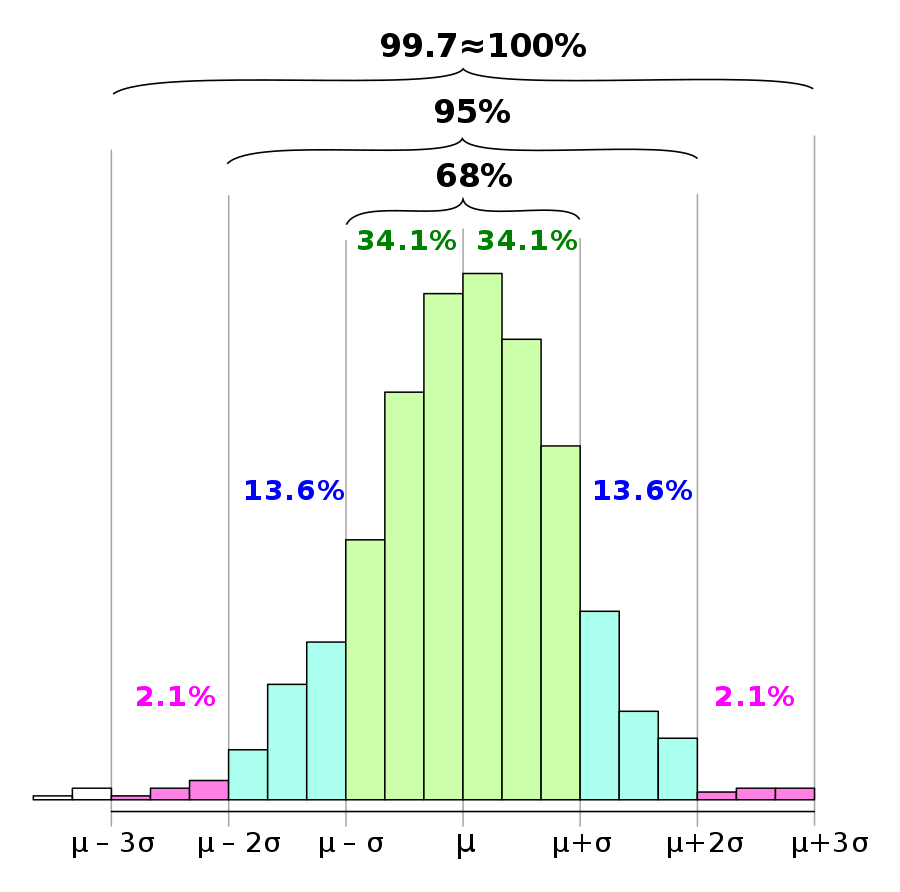
\includegraphics[width=0.5\linewidth]{figs/nsigma_wiki}
  \caption{A test sampling from Gaussian (normal) distribution (from Wikimedia).}
  \label{fig:nsigmawiki}
\end{figure}

In this sense, the ``$ n $-$ \sigma $'' is defined as the $ x $-axis value which gives the integrated area of certain value. More precisely, we have to call this confidence interval (CI):

\begin{defn}[$ n $-$ \sigma $ Confidence Interval; CI]
  1-$ \sigma $ CI is the integrated area is $ 0.6827\cdots $ of the total area. Similarly, 2-$ \sigma $ CI is that with $ 0.9545\cdots $, 3-$ \sigma $ CI is that with $ 0.9973\cdots $, etc. 
\end{defn}

Mathematically it is more correct to call, e.g., 1-$ \sigma $ CI as the $ 68.27\cdots \% $ CI. We also define the significance level $ \alpha $ as 100\% minus this percentage, i.e., the 1-$ \sigma $ CI is of significance level $ \alpha = 1 - 0.6827\cdots = 0.3173\cdots $:
\begin{equation}
  \text{1-}\sigma \text{ CI}
  \quad \equiv \quad 
  68.27\cdots \% \text{ CI}
  \quad \equiv \quad 
  \text{CI of significance level } 0.3173 \cdots ~.
\end{equation}
In natural sciences we often use $ n $-$ \sigma $ CI, but in mathematics and other branches of sciences and engineering, the 90 \%, 95 \%, and 99 \% CIs, i.e., CIs with significance level $ \alpha = 0.10,\, 0.05,$ and $ 0.01 $ are used more often.

Because when we say ``$ n $-$ \sigma $'', we are just omitting the term ``CI'' at the end of it, this is not $ n $ times the standard deviation ($ \sigma $): What we mean by ``$ n $-$ \sigma $'' is actually ``$ n $-$ \sigma $ CI'' and is \textit{not necessarily} $ n \times \sigma $. 

They are the same for, e.g., Gaussian distribution. For Gaussian (normal) distribution, which is a distribution that appears very often in natural sciences, such a 2-$ \sigma $ is nothing but 2 times the standard deviation ($ \sigma $). For almost all of the distributions other than Gaussian, this is not the case.



\section{The Meaning of $ \pm $ Sign}
Simple answer: The $ \pm $ sign means the 1-$ \sigma $ confidence interval (CI). It is also simply called as the ``error-bar''. 

Honestly speaking, the $ \pm $ sign, i.e., the 1-$ \sigma $ CI, does \textit{not} fully describe the uncertainty. The best way to show or describe the uncertainty is to show a graph of probability distribution function (pdf or p.d.f.) as in \cref{fig:figposterior01}. In many but not all publications or books, people do not show this, because (1) the distribution is very similar to Gaussian or certain widely known distribution and it is clearly written in the text or assumed as all the readers know that, (2) detailed calculation is not of interest and/or does not affect the final result, (3) the writer is lazy. 

\begin{figure}[ht!]
\centering
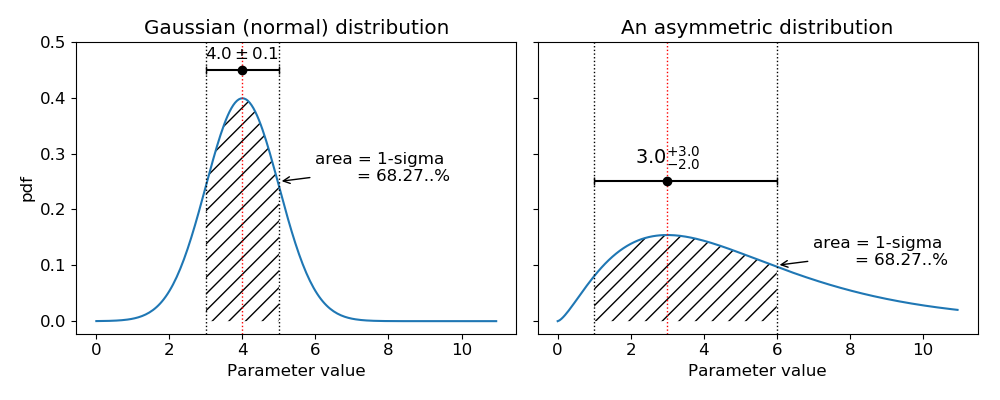
\includegraphics[width=1\linewidth]{figs/fig_posterior01}
\caption{The probability distribution function (pdf) of two examples of distributions, namely, Gaussian and an asymmetric distributions. I used a chi-square distribution for the latter for plotting purpose.}
\label{fig:figposterior01}
\end{figure}


The uncertainty ranges shown in the figure ($ 4.0 \pm 0.1 $ and $ 3.0^{+3.0}_{-2.0} $) are determined such that the lower/upper bounds include $ 68.27 \cdots \% $ of the total area. It is trivial for a Gaussian distribution: mean $ \pm $ 1-$ \sigma $. But if the distribution is asymmetric (right panel of the figure), there are few choices to set such bounds. First and the most widely used one is to set the bounds such that the distance between upper/lower bounds are minimized (but include $ 68.27 \cdots \% $ of the total area). Second is to make it symmetric while include $ 68.27 \cdots \% $ of the total area, so that you can use $ \pm $ sign for simplicity ($ 3.0 \pm 2.\mathrm{XX} $ for example). Third choice would be something like FWHM: find $ x $-axis values such that the pdf value is $ 0.5 \times \mathrm{pdf_{max}} $. The last two bounds are simple to calculate but not as accurate as the first choice.

Very assymetric probability distributions appear in cosmological sciences\footnote{Google ``posterior distribution cosmological constants''.} and exhaustive statiscal analyses are conducted on such models to reject cosmological models. The reason is that, in cosmology, we have only one single sample (our universe), and the statistical analyses given the observational data is of utmost importance. Of course similar exhaustive statistical analyses should be conducted on any research field if the data/object/target is of such importance. 



\section{Caveat on the ``$ n $-$ \sigma $ CI'' Notation}
Let me emphasize again: What we mean by ``$ n $-$ \sigma $'' is actually ``$ n $-$ \sigma $ CI'' and is \textit{not necessarily} $ n \times \sigma $. 

It maybe is tempting to convert the 1-$ \sigma $ CI to the 3-$ \sigma $ CI. For instance, from \cref{fig:figposterior01}, $ 4.0 \pm 0.1 $ and $ 3.0^{+3.0}_{-2.0} $ to $ 4.0 \pm 0.3 $ and $ 3.0^{+9.0}_{-6.0} $. This is true for the former (Gaussian) but wrong for the latter (non-Gaussian). The lower bound of the second parameter now become negative ($ 3.0 - 6.0 = -3.0 $), which is not even physically correct if this parameter is defined to be positive. What you have to do is, get the 3-$ \sigma $ CI which should contain $ 0.9973\cdots $ of the total area from the distribution given in \cref{fig:figposterior01}. There can be at least three choices to do it, which I mentioned in the previous section.


\section{Central Limit Theorem (CLT)}
The Central Limit Theorem (CLT) is at the heart of all the observational or experimental sciences. It is stated as\footnote{For strict definitions of random sample, population, independence, the statement of CLT in mathematical senses, etc, I recommend mathematical statistics textbooks.}

\begin{thm}[Central Limit Theorem; CLT] \label{thm: clt}
  Consider a random sample (observation, measurement, etc) with size $ n $ and the mean value of this sample is $ \bar{X} $. Then $ (\bar{X} - \mu) / (\sigma / \sqrt{n}) $ approaches the standard normal distribution ($ \mathcal{Z} $) as $ n \rightarrow \infty $, where $ \mu $ and $ \sigma^2 $ are the (finite) mean and variance of the population:
  \begin{equation}
    \frac{\bar{X} - \mu}{\sigma / \sqrt{n}} \sim \mathcal{Z}  \quad (\mathrm{as~} n \rightarrow \infty)~.
  \end{equation}
\end{thm}

There is one more important theorem, which we usually skip to mention:

\begin{thm}[Sample Variance Distribution] \label{thm: s and sigma}
  Consider a random sample (observation, measurement, etc) with size $ n $ and the sample variance is $ S^2 $. Then $ (n - 1) S^2 / \sigma^2 $ follows a chi-squared distribution with degrees of freedom $ (n - 1) $, where $ \sigma^2 $ is the variance of the population:
  \begin{equation}
    \frac{(n - 1) S^2}{\sigma^2 } \sim \chi^2_{(n-1)}
  \end{equation}
\end{thm}

Also the definition of the Student $ t $-distribution\footnote{This definition is directly copied from Walpole et al. p.177}:

\begin{defn}[Student $ t $-distribution]\label{def: t-distn}
  Let $ Z $ be a standard normal random variable and $ V $ a chi-squared random variable with $ v $ degrees of freedom. If $ Z $ and $ V $ are independent, then the distribution of the random variable $ T $, where
  \begin{equation}
    T = \frac{Z}{\sqrt{V /v}}
  \end{equation}
  is given by the density function
  \begin{equation}
    h(t) = \frac{\Gamma \qty[ \frac{v+1}{2} ]}{\Gamma \qty[\frac{v}{2}] \sqrt{\pi v}}
      \qty( 1 + \frac{t^2}{v} )^{-\frac{(v+1)}{2}}
    \quad ~, \quad
    -\infty < t < \infty ~.
  \end{equation}
  This is known as the Student $ t $-distribution with $ v $ degrees of freedom.
\end{defn}

We can see that the $ t $-distribution approaches the standard normal distribution as the degrees of freedom $ v \rightarrow \infty $, because the power term takes the $ e^{-t^2 / 2} $ form. 


\begin{thm}[Practical Usage of the CLT] \label{thm: practical clt}
  Consider a random sample (observation, measurement, etc) with size $ n $ large enough and the mean value of this sample is $ \bar{X} $. If $ \mu $, $ \sigma^2 $, and $ S^2 $ are the (finite) mean and variance of the population, and the sample variance, respectively:
  \begin{equation}
    \frac{\bar{X} - \mu}{S / \sqrt{{n}}} \sim T_{(n - 1)} ~.
  \end{equation}
\end{thm}

Sometimes people empirically say $ n \ge 30 $ is enough. This really depends on the situation and I will skip this issue here. The sketch of the proof of the theorem is simple. By the definition of the $ t $-distribution and Thm \ref{thm: s and sigma}, 
\begin{equation}
  T = \frac{Z}{\sqrt{V /v}} = \frac{ \frac{\bar{X} - \mu}{\sigma / \sqrt{n}} }
  {\sqrt{ \frac{(n - 1) S^2}{\sigma^2 } / (n-1)}}
  = \frac{\bar{X} - \mu}{S / \sqrt{{n}}}
\end{equation}
so the theorem is plausible. For your information, the sample variance is defined as
\begin{equation}
  S^2 := \frac{1}{n - 1} \sum_{i=1}^{n} (X - \bar{X})^2 
\end{equation}
and the sample standard deviation $ S $ is the square root of this.

Note here the difference between Thm \ref{thm: clt} and Thm \ref{thm: practical clt}: $ \sigma $ is changed to $ S $, and the standard normal distribution is changed to the $ t $-distribution of $ (n - 1) $ degrees of freedom. Since the true variance $ \sigma^2 $ is unknown, it is difficult to use the CLT (Thm \ref{thm: clt}) directly. But thanks to Thm \ref{thm: s and sigma}, we can use the variance of the sample, $ S^2 $, which is measurable, and utilize the $ t $-distribution, which is slightly bothersome than the standard normal distribution but still useful. 

Also be aware that CLT says the \textit{expectation value of the mean} is normally distributed, not the \textit{sample} is so.

\begin{ex}[Coin Tossing and the CLT]
  Consider a coin-tossing experiment and assign $ \pm 1 $ to heads and tails. Each experiment will give you $ \pm 1 $, but never $ 0 $. Meanwhile, we know a fair coin should have $ \mu = 0 $ (same probability of heads and tails). After $ n = 100 $ experiments, say you obtained $ \bar{X} = 0.01 $ and $ S = 0.1 $, so
  \begin{equation*}
    T = \frac{\bar{X} - \mu}{S / \sqrt{{n}}}
      = \frac{0.01 - \mu}{0.1 / \sqrt{100}} 
      = 1 - 100 \mu ~.
  \end{equation*}
  Since $ T \sim t_{99} $, the significance level $ \alpha = 0.05 $ confidence interval, i.e., the confidence interval containing $ 100 (1 - \alpha) \% = 95 \% $, can be
  \begin{equation*}
    t_{99, 0.025} < T < t_{99, 0.975}
    \quad \rightarrow \quad
      - 1.9842 < 1 - 100 \mu < 1.9842
    \quad \rightarrow \quad
      \mu \in [-0.0098,\, 0.0298] ~.
  \end{equation*}
  The notation $ t_{\nu, x} $ means the input argument of the $ t $-distribution with the degrees of freedom $ \nu $ such that $ \int_{-\infty}^{t_{99, x}} h(t) dt = x $. Thus, to get the two-tail CI of significance level $ \alpha $, we need to calculate $ t_{\nu, \alpha / 2} $ and $ t_{\nu, 1 - \alpha / 2} $. For a symmetric distribution like $ t $ here, $ t_{\nu, 1 - \alpha / 2} = - t_{\nu, \alpha / 2} $. This is very widely used standard notation.
  
  If you just calculated without pondering about the meaning of the caculation, you may be surprised that your next experiment gives either $ +1 $ or $ -1 $, while the expectation is $ \mu \in [-0.0098, 0.0298] $. This is because the result from CLT is, as described, about the \textit{mean} of the samples, not the \textit{single sample}. Thus, the error-bar from the CLT is not necessarily predicting the possible range of \textit{future experiments}, but it just confines the \textit{position of the mean}.
\end{ex}
The range which predicts the future experiments is called the prediction interval. You may learn the prediction interval (PI) to clarify this difference.

The two-tail significance level $ \alpha $ interval of the $ t $-distribution calculable in python by
\begin{python}
from scipy.stats import t
alpha = 0.95
nu = 99

# Note that the alpha below is NOT the significance level, 
# but the area under the curve!
lo, hi = t.interval(alpha=alpha, df=nu)
print(f"Confidence Interval: [{lo:.4f}, {hi:.4f}]")
\end{python}


\subsubsection*{Note: Uncertainty of Median}
The 1-$ \sigma $ error-bar of the median is more difficult to handle than that of the mean (CLT: Thm \ref{thm: clt}). But we can get a result from simplifying assumptions, which are not necessarily true for real observations:

\begin{thm}[Uncertainty of Median]
  Consider $ n (\gg 1) $ samples are independently drawn from $ X \sim \mathcal{G}(\mu, \sigma^2) $, a general continuous distribution with finite mean and variance $ \mu $ and $ \sigma^2 $ with pdf $ p(x) $. The uncertainty of the median estimator is 
  \begin{equation}\label{eq: err median general}
    \Delta \mathrm{med} \approx \frac{1}{2 p(\nu_0) \sqrt{n - 1}}
  \end{equation}
  and if $ \mathcal{G} =  \mathcal{N} $, i.e., a normal distribution,
  \begin{equation}\label{eq: err median}
    \Delta \mathrm{med} 
      \approx \sqrt{\frac{\pi / 2}{n - 1}} s 
      = \sqrt{\frac{\pi}{2} \frac{n}{n - 1}} \Delta \mathrm{mean}
      \approx 1.25 \Delta \mathrm{mean}
       ~,
  \end{equation}
  where $ s $ is the sample standard deviation and $ \Delta \mathrm{mean} = s / \sqrt{n} $ is the error-bar of the mean from Thm \ref{thm: practical clt}.
\end{thm}
\begin{proof}[of general distribution]
To prove it, say the true median is $ \nu_0 $ and samples $ \{ x_1, \cdots, x_n \} $ are sorted as increasing order. For an integer $ m $, set $ n = 2m + 1 $, because $ n \gg 1 $. The sample median is then $ \nu = x_{m + 1} $.
The probability of having sample median $ \nu $ is calculable by noting that we have to sample $ m $ of sample with $ x_i \le \nu $ and the other $ m $ with $ x_i > \nu $:
\begin{equation*}
  f(\nu) = \frac{n!}{m! m!} q^m (1 - q)^{m} ~,
\end{equation*}
where $ q = q(\nu) = \mathbb{P} \{ X_i \le \nu \} = \int_{-\infty}^{\nu} p(x) dx $. $ p(x) $ is the pdf of the normal distribution. 

The Taylor expansionof $ q $ at $ \nu = \nu_0 $:
\begin{equation*}
\begin{aligned}
  q(\nu) &= q(\nu_0) + \frac{1}{1!} q'(\nu_0) (\nu - \nu_0) + O\qty( (\nu - \nu_0)^2 )\\
    &\approx \frac{1}{2} + q'(\nu_0) (\nu - \nu_0) \\
    &\equiv \frac{1}{2} + p(\nu_0) (\nu - \nu_0) ~.
\end{aligned}
\end{equation*}
Then 
\begin{equation*}
\begin{aligned}
  f(\nu) &\approx \frac{n!}{m! m!}
    \qty[ \frac{1}{2} + p(\nu_0) (\nu - \nu_0) ]^m
    \qty[ \frac{1}{2} - p(\nu_0) (\nu - \nu_0) ]^m \\
    &= 
    \frac{n!}{m! m!}
    \qty[ \frac{1}{4} \qty( 1 - 4 p(\nu_0)^2 (\nu - \nu_0 )^2) ]^m \\
    &= 
    \frac{n!}{m! m! 4^m}
    \qty[ 1 - \frac{4 m p(\nu_0)^2 (\nu - \nu_0 )^2}{m} ]^m \\
    &\approx 
    \frac{n!}{m! m! 4^m}
    e^{ -4 m p(\nu_0)^2 (\nu - \nu_0 )^2 } ~.
\end{aligned}
\end{equation*}
This has the form of Gaussian distribution ($ \propto e^{-(x - \mu)^2 / 2\sigma^2} $) with mean $ \nu_0 $ and variance $ \frac{1}{4 (n-1) p(\nu_0)^2} $ since $ m = (n - 1) / 2 $. Thus, 
\begin{equation}
  \nu \sim \mathcal{N} \qty( \nu_0, \frac{1}{4 (n-1) p(\nu_0)^2} )
  \quad\rightarrow \quad
  \Delta \mathrm{med} \approx \frac{1}{2 p(\nu_0) \sqrt{n - 1}} ~.
\end{equation}
Q.E.D.
\end{proof}

\begin{proof}[of Gaussian distribution]
Now if $ p(x) $ is a Gaussian, median is equal to mean, so the pdf becomes $ p(\nu_0) = p(\mu) = \frac{1}{\sqrt{2\pi} \sigma} $, and
\begin{equation*}
  \nu \sim \mathcal{N} \qty( \nu_0, \frac{\pi / 2}{n - 1} \sigma^2 ) ~.
\end{equation*}
If we denote $ A = \sqrt{(n - 1) / (\pi / 2)} $, the statistic $ Z = A \frac{\nu - \nu_0}{\sigma} $ will follow the standard normal distribution. On the other hand, $ V = \frac{(n - 1) s^2}{\sigma^2} $ follows the chi-squared distribution of degrees of freedom $ (n - 1) $ by Thm \ref{thm: s and sigma}. Then 
\begin{equation*}
  T = \frac{Z}{\sqrt{V / (n - 1)}}
    = A \frac{\nu - \nu_0}{s}
\end{equation*}
will follow a $ t $-distribution with degrees of freedom $ (n - 1) $ by Def \ref{def: t-distn}. $ T $ is nearly a Gaussian when $ n $ is large (rule-of-thumb: when $ n \gtrsim 30 $), so 
\begin{equation}
  \nu \mathrel{\dot{\sim}} \mathcal{N} \qty( \nu_0, \frac{\pi / 2}{n - 1} s^2 )
  \quad\rightarrow \quad
  \Delta \mathrm{med} \approx \sqrt{\frac{\pi / 2}{n - 1}} s  ~.
\end{equation}
Q.E.D.
\end{proof}



\section{Meaning of the Confidence Interval}
I circunvented the definition of the CI so far. It is defined as

\begin{defn}[Confidence Interval; CI] 
  A confidence interval of significance level $ \alpha $ of a parameter $ X $ is the interval of $ X $ value such that if we conduct the identical parameter estimation process in many \textit{parallel universes} (i.e., ensemble) which have the identical true value $ X_\mathrm{true} $, fraction of $ (1 - \alpha) $ of such universes could have calculated a CI such that the $ X_\mathrm{true} $ is included in that CI.
\end{defn}

This is not a practically meaningful definition, but philosophically important. Let me give an example to elaborate the meaning of this.

\begin{ex}[Meaning of the Confidence Interval]
  Imagine there are many \textit{parallel universes} and the same observer observes the same star in each universe. Because of random errors (which we will learn later but that includes Poisson photon noise, readout noise, etc), the observer at each universe will obtain slightly different observational results. The observers will observe the star for $ n $ times, and calculate their own mean and error-bar as $ \bar{X} $ and $ S / \sqrt{n} $ from their observations. Note again that  $ S / \sqrt{n} $ is the uncertainty of the \textit{mean} value.

  For visualization, the true magnitude of the star is $ \mu = \m{14.0} $ and true standard deviation of the observation $ \sigma = \m{0.2} $ with $ n = 9 $ are used for the generation of \cref{fig:figclt01}. The universe ID 0 of both the upper and lower panels show roughly $ m = \m{14.0} \pm \m{0.1} $. That is, when the true magnitude and true standard deviation are given as $ \m{14.0} $ and $ \m{0.2} $, an observer at one of the universes (in our case universe ID 0) got $ m = \m{14.0} \pm \m{0.1} $, and that is our universe. 
\end{ex}

\begin{figure}[ht!]
  \centering
  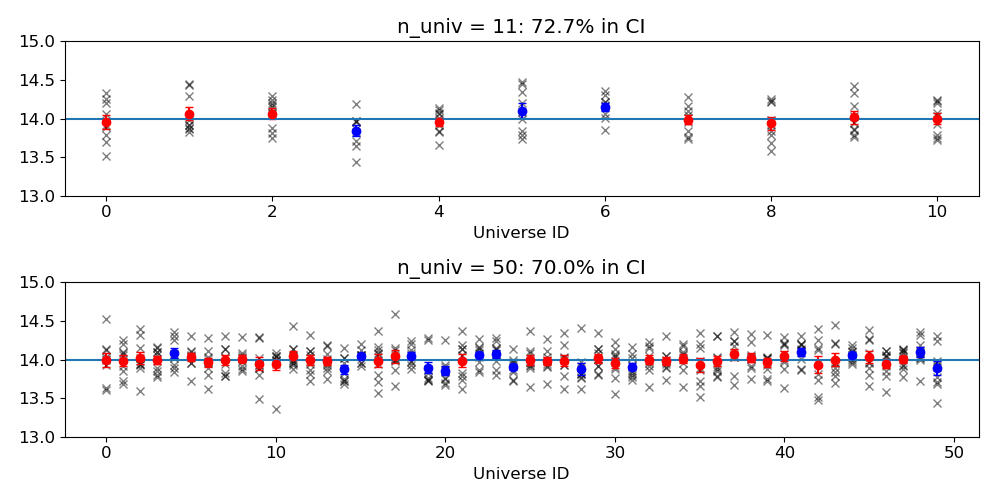
\includegraphics[width=1\linewidth]{figs/fig_clt01}
  \caption{Simulation to show the concept of CI and CLT. Black crosses are the observation in each universe, and the circles are the mean and its uncertainty from the CLT $ S / \sqrt{n} $. Red circles are the univserses where the confidence interval contains the true mean $ \mu = \m{14.0} $ and blue circles are the others. In the title, the fraction of the universes which contains the true mean within their own confidence intervals out of \texttt{n\_univ} simulated universes is shown. This fraction approaches $ 0.6827\cdots $ as the number of universe gets infinity.}
  \label{fig:figclt01}
\end{figure}

I will close this section with an excerpt from Walpole p.234:

\textit{The interpretation of a CI is often misunderstood. It is tempting to conclude that the parameter falls inside the CI with probability of(, e.g.,) 0.95. (But this is not ture.) A CI merely suggests that if the experiment is conducted and data are observed again and again, about 95\% of such intervals will contain the true parameter.}



\section{Answer to the Question}
In statistics, the \textit{null hypothesis}, denoted $ H_0 $, is the one that is the simplest, and that has value if it is \textit{rejected} (not \textit{accepted}). The \textit{alternative hypothesis}, $ H_1 $, is another possibility if $ H_0 $ is not true. In the simplest case, $ H_1 $ is the complementary of $ H_0 $. For example, $ H_0: \mu = 0 $ and $ H_1: \mu \neq 0 $. 

Let's consider the opening question: $ m = \m{14.0} \pm \m{0.1} $. Now you understand that $ \m{14.0} $ means that the mean value\footnote{It can actually be the median value, most probable value, or whatever the representative value.} from the observation, and $ \pm \m{0.1} $ means the uncertainty or the error-bar of the Gaussian probability distribution of that mean value, $ S / \sqrt{n} $. If it were not Gaussian, the author should have given more information. Note that the sample standard deviation is $ \sqrt{n} $ times the error-bar.

To answer the question, we set the hypotheses\footnote{There are some ``standard'' ways to set the hypotheses, and it may seem very sudden if you are not familiar with these. Please refer to basic applied statistics textbooks for more examples, e.g., p.246 and p.264 of Walpole et al.}:
\begin{equation}
  H_0 : m_1 = m_2 
  \sep
  H_1 : m_1 \neq m_2 ~,
\end{equation}
where $ m_1 = \m{14.0} \pm \m{0.1} $ and $ m_2 $ is the other (from researcher 2). $ m_1 $ and $ m_2 $ here means the ``true'' magnitude of the star, not the measured value! If it were the measured value, they are just different, since one is 14.0 and the other is 15.0. The two true means may be different because (1) researchers may have mistakenly observed different star, (2) the star is maybe a variable (including binary), (3) explanet occulted some part of the star, or any other scenario is possible.

Now we have to choose which formula to use. When two measurements with $ \bar{x}_1 \pm s_1 $ and $ \bar{x}_2 \pm s_2 $ from the number of observations $ n_1 $ and $ n_2 $ are given, and $ \mu_1 $ and $ \mu_2 $ are the true means of two sampling distributions that will be tested under the hypothesis testing, there are two different formulae:
\begin{itemize}
\item The true variances are unknown and different (Satterthwhite approximation\footnote{SatterthwhiteFE (1946, Biometrics Bulletin, 2, 110), ``An Approximate Distribution of Estimates of Variance Components.''}):
\begin{equation}
  t = \frac{(\bar{x}_1 - \bar{x}_2) - (\mu_1 - \mu_2) }{\sqrt{s_1^2 / n_1 + s_2^2 / n_2}}
\end{equation}
follows the $ t $-distribution with degrees of freedom
\begin{equation}
  \nu \approx 
    \frac{\qty( s_1^2 / n_1 + s_2^2 / n_2 )^2}
    {\frac{ \qty(s_1^2 / n_1)^2 }{n_1 - 1}
      + \frac{ \qty(s_2^2 / n_2)^2 }{n_2 - 1}} ~.
\end{equation}
\item The true variances are unknown but the same:
\begin{equation}
  t = \frac{(\bar{x}_1 - \bar{x}_2) - (\mu_1 - \mu_2) }{s_p \sqrt{1 / n_1 + 1 / n_2}}
\end{equation}
follows the $ t $-distribution with degrees of freedom $ \nu = n_1 + n_2 - 2 $ and
\begin{equation}
  s_p = \frac{(n_1 - 1) s_1^2 + (n_2 - 1) s_2^2}{\nu} ~.
\end{equation}
\end{itemize}
Which one will you choose? To answer our original question, it is more reasonable to assume the true variances are not necessarily identical, because they may have used different instruments at different sky conditions. So I will use the first choice.

To apply the formula, you need the number of observations from each researcher, i.e., the $ n_1 $ and $ n_2 $ values. As I mentioned, it is an ill-defined question since this numbers are not given. So let me assume $ n_1 = n_2 = n = 5 $. The question can be reformulated as $ \bar{x}_1 = 14.0 $, $ \bar{x}_2 = 15.0 $, $ s_1 = 0.1 \sqrt{n} $, and $ s_2 = 1.0\sqrt{n},\, 0.3\sqrt{n}, \, 0.1\sqrt{n} $, where I dropped the magnitude sign for brevity. Under the null hypothesis ($ H_0: \mu_1 = \mu_2 $), $ \mu_1 - \mu_2 = 0 $. For the three $ s_2 $ values, 
\begin{equation}
\begin{aligned}
  t &= \frac{(14.0 - 15.0) - 0}{\sqrt{(s_1^2 + s_2^2) / n}}
  \quad &&\rightarrow \quad
  t &&= & -0.995 ,\, && -3.162 ,\, && -7.07 \\
  \nu &= (s_1^2 + s_2^2) (n-1)
  \quad &&\rightarrow \quad
  \nu &&= & 4.08, \, && 4.32, \, && 8.0 \\
  &&&&&\approx & 4 ,\, && 4 ,\, && 8 \\
\end{aligned}
\end{equation}
The values are in the order for $ s_2 = (1.0,\, 0.3, \, 0.1)\sqrt{n} $ cases. The (two-tail) significance level $ \alpha $ test is listed in \cref{tab: CI}.

\begin{table}[ht!]
\centering
\caption{The confidence interval calculation for the example question.}
\label{tab: CI}
\begin{tabular}{c|c||c|c}
CI \% & significance level $ \alpha $ and $ \frac{\alpha}{2} $& $ \nu = 4 $ case & $ \nu = 8 $ case \\
\hline
90 \% & 0.10 \& 0.05   & $ [-2.1318, 2.1318] $ & $ [-1.8595, 1.8595] $ \\
95 \% & 0.05 \& 0.025  & $ [-2.7764, 2.7764] $ & $ [-2.3060, 2.3060] $ \\
99 \% & 0.01 \& 0.005  & $ [-4.6041, 4.6041] $ & $ [-3.3554, 3.3554] $ \\
\end{tabular}
\end{table}

The answers to the questions are, assuming $ n_1 = n_2 = 5 $,
\begin{itemize}
\item Case A ($ t = -0.995 $ with $ \nu = 4 $): The $ t $ value is inside of all three CIs. Thus, we cannot reject $ H_0 $ under 90 \%, 95 \%, and 99 \% CI criterion (cannot reject under the significance level $ \alpha = 0.10,\, 0.05,\, 0.01 $).
\item Case B ($ t = -3.162 $ with $ \nu = 4 $): The $ t $ value is inside of 90 \% and 95 \% CI but outside of the 99 \% CI. Thus, we reject $ H_0 $ with $ \alpha = 0.10 $ and $ 0.05 $, but cannot reject it with $ \alpha = 0.01 $.
\item Case C ($ t = -7.07 $ with $ \nu = 8 $): We reject $ H_0 $ with all the three $ \alpha = 0.10,\, 0.05,\, 0.01 $.
\end{itemize}
\vspace{\parskip}

By \textit{rejecting the null hypothesis}, $ H_0: m_1 = m_2 $, we mean that it is unlikely that the true magnitude value of the two studies are identical. By \textit{failing in rejecting the null hypothesis}, we mean that it is impossible to conclude whether $ m_1 $ and $ m_2 $ are the same under the given significance level. 

The results are as expected: For Case A, the error-bar of $ m_2 $ is too large, which means it is almost impossible to reject the claim that $ m_1 = m_2 $, so the we always fail to reject the null hypothesis. For Case C, the error-bars are too small and thus $ m_1 $ is of course vastly different from $ m_2 $, so the null hypothesis is always rejected.

%\footnote{You may wonder what if we have $ n = 1 $. The $ \nu $ is undetermined and all the calculation seem to meaningless, but of course we can have error-bars for each single observation. That is not considered in this example since here we are simply assuming the mean is inferred from $ n $ observations under the CLT, and we need $ n > 1 $ to calculate the sample variance $ S^2 $. I will not consider the error-bars of each observations. Such a detailed statistical analyses should follow some well-developed and specific statistical routines available in your research field.}.
%In this example we do not care about the error-bar of each observation but the final error-bar of the mean value from researchers. If we want to consider the error-bars of every observations, this kind of classical statistical method gets very complicated and almost impossible to give meaningful results. You then need Bayesian approach and Monte Carlo simulation technique.




\section{Poisson Noise}
The Poisson process is a fancy naming for some special ``counting''. In astronomy, we count photons (well, actually the CCD counts the electrons) over time, in social sciences we can count the death toll over time, in experiments we could count the lattice of a randomly shaped crystal over the distance. A formal definition is\footnote{See, e.g., \url{http://dept.stat.lsa.umich.edu/~ionides/620/notes/poisson_processes.pdf} and \url{https://www.probabilitycourse.com/chapter11/11_1_2_basic_concepts_of_the_poisson_process.php}}

\begin{defn}[Poisson Process 1]
The Poisson process $ N(t) $ for $ t \ge 0 $ ($ t $ can be time, distance, or similar things), with rate $ \lambda $ is defined by
\begin{enumerate}
\item $ N(0) = 0 $
\item $ N(t) $ has independent increment
\item $ N(t_2) - N(t_1) $ follows Poisson distribution of rate $ \lambda (t_2 - t_1) $ for $ t_1 < t_2 $.
\end{enumerate}
\end{defn}

It can be proven that it is identical to 

\begin{defn}[Poisson Process 2]
The Poisson process $ N(t) $ for $ t \ge 0 $ ($ t $ can be time, distance, or similar things), with rate $ \lambda $ is defined by
\begin{enumerate}
\item $ N(0) = 0 $
\item $ N(t) $ has independent increment
\item $ \mathbb{P}(N(h) = 1) = \lambda h + o(h) $ for small $ h $.
\item $ \mathbb{P}(N(h) \ge 2) = o(h) $ for small $ h $.
\end{enumerate}
\end{defn}

Here $ o(h) $ is any function such that $ \lim_{h \rightarrow 0} o(h) / h = 0 $. The last two items in this second definition can be re-phrased like this:
\begin{itemize}
\item [3.] For a very small interval $ h $, the probability of one single ``counting'' (Poisson process) occurs in that interval is proportional to the length of $ h $.
\item [4.] For a very small interval $ h $, the probability of two or more ``counting'' (Poisson process) occurs in that interval is nearly 0.
\end{itemize}
These must be independent of whether the counting happened outside of the interval, because the second item of the definition states the increment is independent.
\newpage
\begin{ex}[Photon Counting and Poisson Process]
The photon counting process of astronomy resembles the Poisson Process. If $ N(t) $ is the number of photons or electrons under the exposure time $ t $, it is trivial that the first two items of the definition is satisfied. Next, use the rephrased version of the next items. The number of photons hitting CCD with infinitesimal time interval $ h = dt $ must be 0 or 1, but not larger than 1 (e.g., if a pixel count is 10,000 after 10 sec of exposure, we can take $ h \ll \SI{10}{s} / 10,000 = \SI{1}{ms} $ to meet this condition). Thus, photon counting is a Poisson process.
\end{ex}

The Poisson process follow the Poisson distribution:

\begin{defn}[Poisson Distribution] \label{def: Pois pdf}
The Poisson process of rate $ \lambda $ has the following pdf
\begin{equation} \label{eq: Pois pdf}
  p(x; \lambda t) = \frac{(\lambda t)^{x}}{x!} e^{-\lambda t}
\end{equation}
for non-negative integer $ x $.
\end{defn}

\begin{thm}[Poisson Distribution Mean and Variance] \label{thm: Pois mean std}
The mean, variance, and the standard deviation of the Poisson distribution $ p(x; \lambda t) $ are
\begin{equation}\label{eq: Pois mean std}
  \mathrm{mean} = \lambda t
  \sep
  \mathrm{var} = \lambda t
  \sep
  \mathrm{std} = \sqrt{\lambda t} ~.
\end{equation}
\end{thm}
The reason we use $ \lambda t $ not just $ \lambda $ is clear from Thm \ref{thm: Pois mean std}: the mean changes as $ t $ changes, and we want to express $ p(x; \mathrm{mean}) $ rather than $ p(x; \mathrm{mean} / t) $. For instance, if the photon influx is $ \lambda = \SI{10}{photons / s} $, the mean of photon count is a function of time as $ \lambda t $, so for $ t = \SI{10}{s} $, the pdf is $ p(x; \SI{100}{photons}) $. If the particles are distributed with mean density along the line of sight $ \lambda = \SI{0.1}{particle / m} $, the mean of particles along the line of sight is a function of the reaching distance $ \lambda d $, so the pdf for $ d = \SI{5}{m} $ is $ p(x; \SI{0.5}{particles}) $. 

\begin{thm}[Poisson to Gaussian] \label{thm: Pois gauss}
As $ x \rightarrow \infty $, the Poisson distribution approaches normal distribution $ \mathcal{N}( \lambda t, \lambda t ) $.
\end{thm}
Although I will omit here, the proof uses Stirling's formula $ x! \approx \sqrt{2\pi x} x^x e^{-x} $ and $ \ln[ (1 + \varepsilon)^{\lambda t (1 + \varepsilon) + 1 / 2 }] \approx \lambda t \varepsilon + \lambda t \varepsilon^2 / 2 $, where $ x = \lambda t ( 1 + \varepsilon ) $ with $ \lambda t \gg 1 $ and $ \varepsilon \ll 1 $. Stirling's formula has relative error of less than 1 \% when $ x = 1 $ and is almost negligible for any $ x $ of interest in many cases. Considering all the approximations in the proof, we can safely assume that Poisson distribution is quite Gaussian (normal) in many astronomical contexts, unless $ x $ is very small ($ \lesssim 10 $..?).

\begin{ex}[Photon Counting and Poisson Noise]
We saw the photon or electron counting is a Poisson process. Thus, we can use \cref{eq: Pois pdf,eq: Pois mean std}. For example, if we collected 10,000 electrons, the 1-$ \sigma $ uncertainty (1-$ \sigma $ CI) or the standard deviation of this counting is $ \sqrt{10,000} = 100 $, so we denote $ N = 10,000 \pm 100 $. Since the $ N $ is large enough, Thm \ref{thm: Pois gauss} says this is just a Gaussian distribution of mean 10,000 and standard deviation 100 (1 \% of the mean). Since magnitude is $ (\mathrm{const}) - 2.5 \lg (\mathrm{count}) $, differentiation gives a first-order estimation of the uncertainty in the magnitude $ \Delta m = -\frac{2.5}{\ln 10} \frac{\Delta (\mathrm{count})}{\mathrm{count}} = \m{0.01} $ (error-bar), which is small enough for some scientific purposes.
\end{ex}

The next example is not directly related to Poisson process, but related to the binomial distribution (Bernoulli process) which has the pdf of $ b(x; n, p) = \binom{n}{x} p^x (1 - p)^{n - x} $ for getting $ x $ outcomes from $ n $ trials with $ p $ probability to have outcome. The pdf of binomial process approaches Poisson pdf with $ p(x; np) $ when $ n \rightarrow \infty $, $ p \rightarrow 0 $ but $ np $ is finite. Thus, the mean, variance, and standard deviation of such binomial distribution is calculabe using Thm \ref{thm: Pois mean std}.
\begin{ex}[Babies in Hospital: Provided by Prof. Jae-Kwang Kim at KAIST]
There are two hospitals A and B. New babies are born as either sex chromosome XX/XY with probability 50:50. Everyday A gives birth to 45 babies and B to 15 babies. Each hospital recorded the number of days when more than 60 \% of babies are girl.
\begin{enumerate}
\item Which hospital will have more such days?
\item With how much confidence can you say so?
\end{enumerate}
\end{ex}


\section{Error Propagation}
When we have to calculate the uncertainty of a parameter derived from other parameters that have their own uncertainties, what we usually use is the \textit{error propagation}. For example, $ \mathrm{g'} = 14.0 \pm 0.1 $ and $ \mathrm{r'} = 15.0 \pm 0.1 $, what is the uncertainty of the $ \mathrm{g' - r'} $ color? Many astronomers will say it is $ -1.0 \pm 0.14 $, where the error here is $ \sqrt{\sigma_\mathrm{g'}^2 + \sigma_\mathrm{r'}^2} $ ($ \sigma $ is the error-bar). If the temperature is $ T = 100 \pm 1 \si{K} $, what is the fractional uncertainty of bolometric luminosity ($ L = \sigma_\mathrm{SB} T^4 $)? Now people will say $ \Delta L / L \approx \frac{4 \sigma_\mathrm{SB} T^3 \Delta T }{\sigma_\mathrm{SB} T^4} = 4 \Delta T / T = 4 \% $. 

This is, however, only an approximation, and in reality, we need more complicated calculation. Note that it is impossible to know how accurate this approximation is, before you conduct detailed calculation. The reason astronomers use it in spite of the pitfall is because most cases we are only interested in the rough estimation of the error-bar.




\section{The Chi-Square Minimization}
You may have heard of it, or simply the \textit{least square} something. Least square or the chi-square minimization is a process to find the set(s) of model parameters which has the biggest (or bigger than threshold) \textit{likelihood} in Bayesian statistics. The set of ``best'' model parameters is the one with the largest likelihood, so we call it the maximum likelihood estimator, \textbf{MLE}.

Consider independent and identically distributed (\textit{i.i.d.}) random variables\footnote{Random variables $ X_{i} $ for $ i = 0, \cdots, N $ are called i.i.d. if they (1) follow identical probability distribution, say $ f(x) $, and (2) $ f(X = x) = f(X_1 = x_1) \times \cdots \times f(X_N = x_N) $, where $ x = (x_1, \cdots , x_N) $ (same for $ X $). }, e.g., flux as a function of $ \lambda $. It is independent because the measurement at each wavelength itself is independent from that of any other wavelength. It is identically distributed because and we will assume each error-bar is Gaussian. The second assumption is not necessarily correct, and actually that happens many times (e.g., flux is Gaussian distributed but magnitude is not, because it is log of Gaussian distribution).


\clearpage
\begin{equation}\label{key}
  P(\mathbf{\theta}|D, I) = \frac{P(D|\mathbf{\theta}, I) P(\mathbf{\theta}|I)}{P(D, I)}
\end{equation}
\begin{equation}\label{key}
  P(\theta|D, I) \propto P(D | \theta, I) P(\theta|I)
\end{equation}

$ (x_i, y_i) $, independent, $ y \sim N(y_i, \sigma_i^2) $
\begin{equation}\label{key}
  \sum_{i} (y_i - f(x_i| \theta))^2
\end{equation}

\begin{equation}\label{key}
  P(D = \{y_i\}) = \Pi_i A e^{-(f(x_i|\theta)-y_i)^2/2\sigma_i^2} 
\end{equation}

\begin{equation}\label{key}
  \ln P(D = \{y_i\}) = \ln A \sum_i -(f(x_i|\theta)-y_i)^2/2\sigma_i^2
\end{equation}
Maximizing $ P $ == maximizing $ \ln P $ == mininizing summation.
\begin{equation}\label{key}
  \chi^2 = \sum_i \frac{(y_i - f(x_i | \theta))^2}{\sigma_i^2}
\end{equation}

% Propagation of Errors
% chi square


\chapter{Idea of Photometry}

\section{The Point-Spread Function (PSF)}

Stars must be point sources. But from our experience, we know that they are never a point, but a usually nearly circular extended sources on the CCD. The image on the CCD when a single perfect point source is imaged, is called the \textbf{point spread function (PSF)}. There are basically two mechanisms responsible for this: diffraction and seeing. Although diffraction can also be a part of seeing, it is somewhat special than others: It is just impossible to eliminate the diffraction, while other sources of seeing can be removed (see below).

\subsection{Diffraction}
When a light ray passes through a finite-sized aperture, diffraction must occur. Due to this, a point source is blurred to a finite size after it passed through an aperture (e.g., telescope or DSLR camera aperture). 

\begin{ex}[Diffraction]
	For $ D = \SI{1}{m} $ in visible ($ \SI{550}{nm} $ wavelength), the diffraction limit is $ 1.22 \frac{\lambda}{D} = \SI{0.14}{arcsec}$. You may be familiar with this formula. Using the proportionality, you can memorize it as $ \theta_\mathrm{min}^{(\SI{550}{nm})} = \frac{0.14}{D\mathrm{[m]}} \mathrm{arcsec}$.
\end{ex}

It is more complicated in reality: the mirrors and other optical instruments located in the optical path affect the final shape of a point source by diffractions. See \cref{fig:psftelescopes} for the examples of simulated PSFs from optics, i.e., when the seeing effects are neglected.

\begin{figure} [htb!]
	\centering
	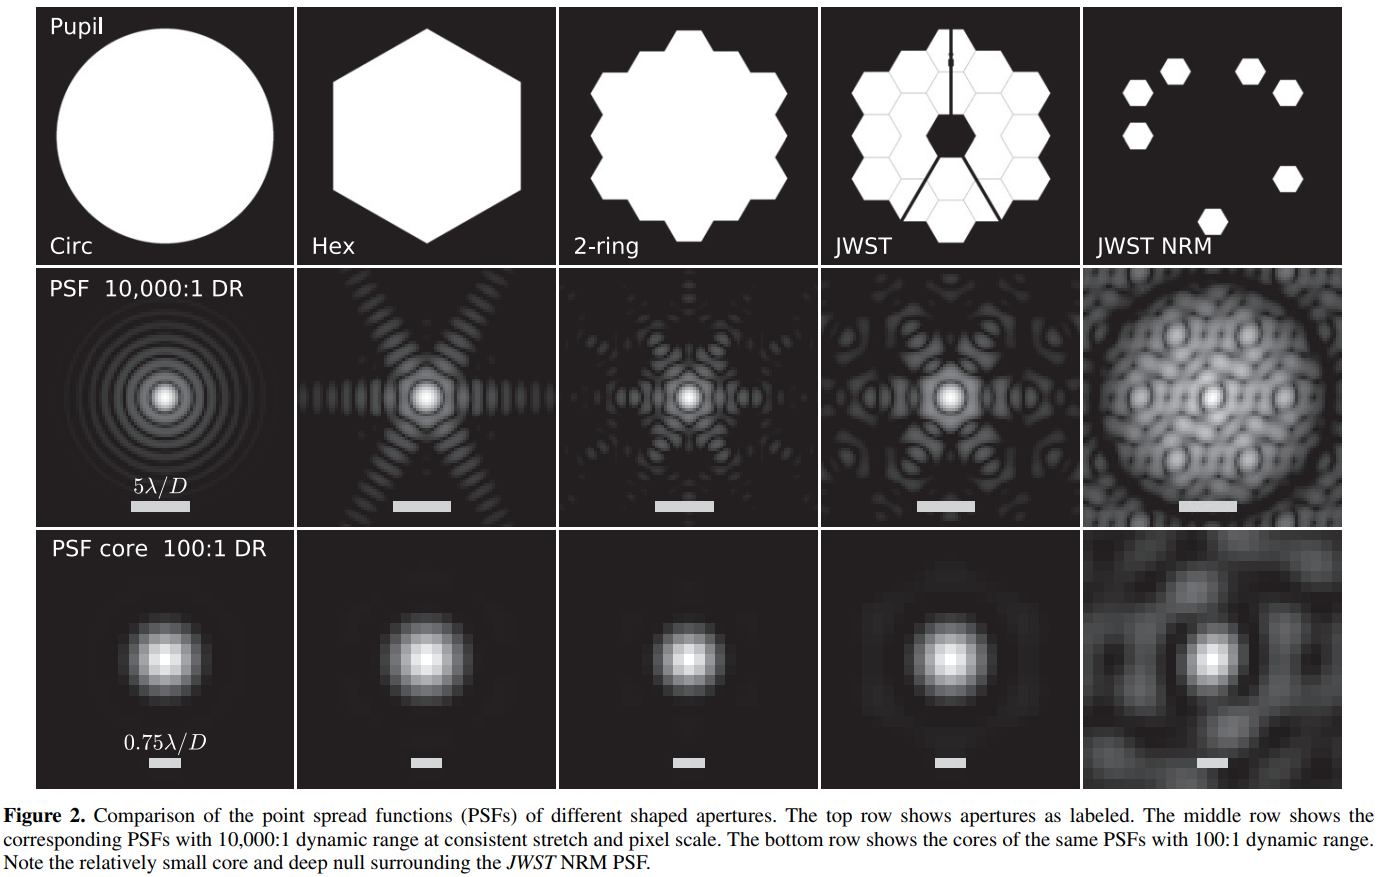
\includegraphics[width=0.9\linewidth]{figs/psf_telescopes}
	\caption{Example of PSFs. For circular aperture, the PSF shows concentric diffraction pattern as we learned in general physics course. For JWST case, you can see the secondary mirror and the mirror holding pipe (black things) makes the PSF different compared to the 2-ring case. The bottom row is not just a zoom-in of the PSF, but also the stretch (contrast) is different from the mid row (DR means the dynamic range). Direct excerpt from Figure 2 of FordKES+, 2014, ApJ, 783, 73.}
	\label{fig:psftelescopes}
\end{figure}

As you can see in \cref{fig:psftelescopes}, although the detailed PSF are different (mid row), the long-range features are weaker compared to the central nearly circular features (bottom row) in cases except for the last column, which is not of our interest. 


\subsection{Seeing}

Even if we ignore the diffraction, a point source is blurred due to two main reasons: (1) air turbulence and (2) discontinuous movement of the telescope since the telescope gear is not a perfectly smooth continuous ideal machine. The blurring caused by these are called \textit{natural (atmospheric)} and \textit{telescopic seeing}, respectively. The atmospheric seeing makes a point source an extended circular source (for details, search for the theory of, e.g., Andrei Kolmogorov), while the telescope seeing \textit{may} make it very elongated or irregular depending on the quality of the tracking system. If the tracking system is well established on a telescope, the final telescope seeing effect is quite circular. 

All these effects can be removed if we move our telescope in space. The atmospheric turbulence is now gone, and the telescope can be very stable such that the telescopic seeing is ignorable. This is what is called the diffraction-limited case.


\subsection{Summary of PSF}

To summarize:
\begin{align*}
  \mathrm{PSF} &= \mathrm{diffraction} + \mathrm{seeing} \\
  \mathrm{seeing} &= \mathrm{atmospheric~seeing} + \mathrm{telescopic~seeing}
\end{align*}
and practically speaking,
\begin{equation*}
  \mathrm{PSF~shape} \approx \mathrm{circular} ~.
\end{equation*}
This is why we can talk about the circular aperture photometry. Also
\begin{align*}
  &\mathrm{diffraction} \ll \mathrm{other~sources~of~seeing} \\ &\mathrm{(unless~adaptive~optics~or~space~telescope~used)} ~.
\end{align*}

Actually, for many ground-based observations, it is not necessarily important to distinguish diffraction from other seeing effects. I feel like people tend to use the word ``PSF'' when the PSF is measured rather accurately (e.g., PSF photometry), and use the word ``seeing'' when we assumed circular PSF (e.g., aperture photometry). 

\subsection{Seeing Disc Size}
As mentioned above, when we assume circular PSF (as we will do frequently in aperture photometry), we use the word ``seeing'' for the PSF. \textit{Seeing disc} is the word for the circular shape of the PSF, and the \textit{seeing disc size} is a measure of the size of that circle. The definition of the ``size'' is not trivial, but many people use the FWHM of the stellar radial profile\footnote{Radial profile means the pixel values of the star image as a function of the distance from the center of the star: $ I(r) $. From many free/commercial products, it is rather easily drawn, such as \texttt{ginga}, \texttt{SAO ds9}, or \texttt{Maxim DL 6}. They also automatically calculates FWHM for you. The details on how to find the ``center'' will be studied later. Here, just think about something like Gaussian curve.}. This seeing disc size measurement is used to find the focal position and give a sense to the data quality.

The seeing disc FWHM is dependent on wavelength, weather, airmass, etc. At Seoul National University observatories in Seoul, it is roughly 1 to 3 arcsec at Bldg. 46 and 3 to 6 arcsec at Bldg. 45. For Subaru telescope at Hawai'i, for example, it is less than 1 arcsec\footnote{\url{https://www.naoj.org/Observing/Telescope/ImageQuality/Seeing/}}. Compared to the diffraction size $ \theta_\mathrm{min} $, these are much larger. It can go even below if we use adaptive optics (then $ \mathrm{diffraction} \approx \mathrm{total~seeing} $ and non-circular PSF may be important).

The fact that the seeing disc size (i.e., size of the circular PSF) on the CCD is normally much larger than the diffraction scale hint that atmospheric and telescope seeing are very important. Since the telescope seeing is roughly constant over time for continuous tracking of a good telescope, the change in seeing can also strongly dependent on the weather condition. So astronomers use seeing disk size (usually rough estimate of FWHM) as a proxy of the weather condition.

It can also be used as a data-quality-indicator.

\begin{ex}[Contamination by Other Object]
If you have your faint target near a bright stellar source with 1 arcsec separation and if the seeing disc FWHM is roughly 1 arcsec, your faint target is contaminated by the nearby bright star. A possibility is to do photometry of ``your target $ + $ bright star'' and subtract the flux of the ``bright star'' from catalog or future/previous observations. In this case, although you can get the flux of the target, its uncertainty may increase significantly. 
\end{ex}

\begin{ex}[Slit Width Determination]
For spectroscopy, seeing disc size may determine the slit width you have to use to collect the target's light into the slit. It will be dealt in the spectroscopy chapter.
\end{ex}

\begin{ex}[Finding Focal Position from Seeing FWHM]
First find a random bright star that do not vary over short period of time (e.g., about 1 hour). You then expose and check the FWHM of the PSF (assuming it is circular). Now tune the focal position, e.g., by moving the position of the secondary mirror, and expose again, and check the FWHM again. Doing this repeatedly, you can get the FWHM as a function of the focal position. When the FWHM becomes the minimum, that is \textit{the} focal position (\cref{fig:focusing}). Normally this curve is roughly second order polynomial.
\end{ex}

\begin{figure}[ht!]
  \centering
  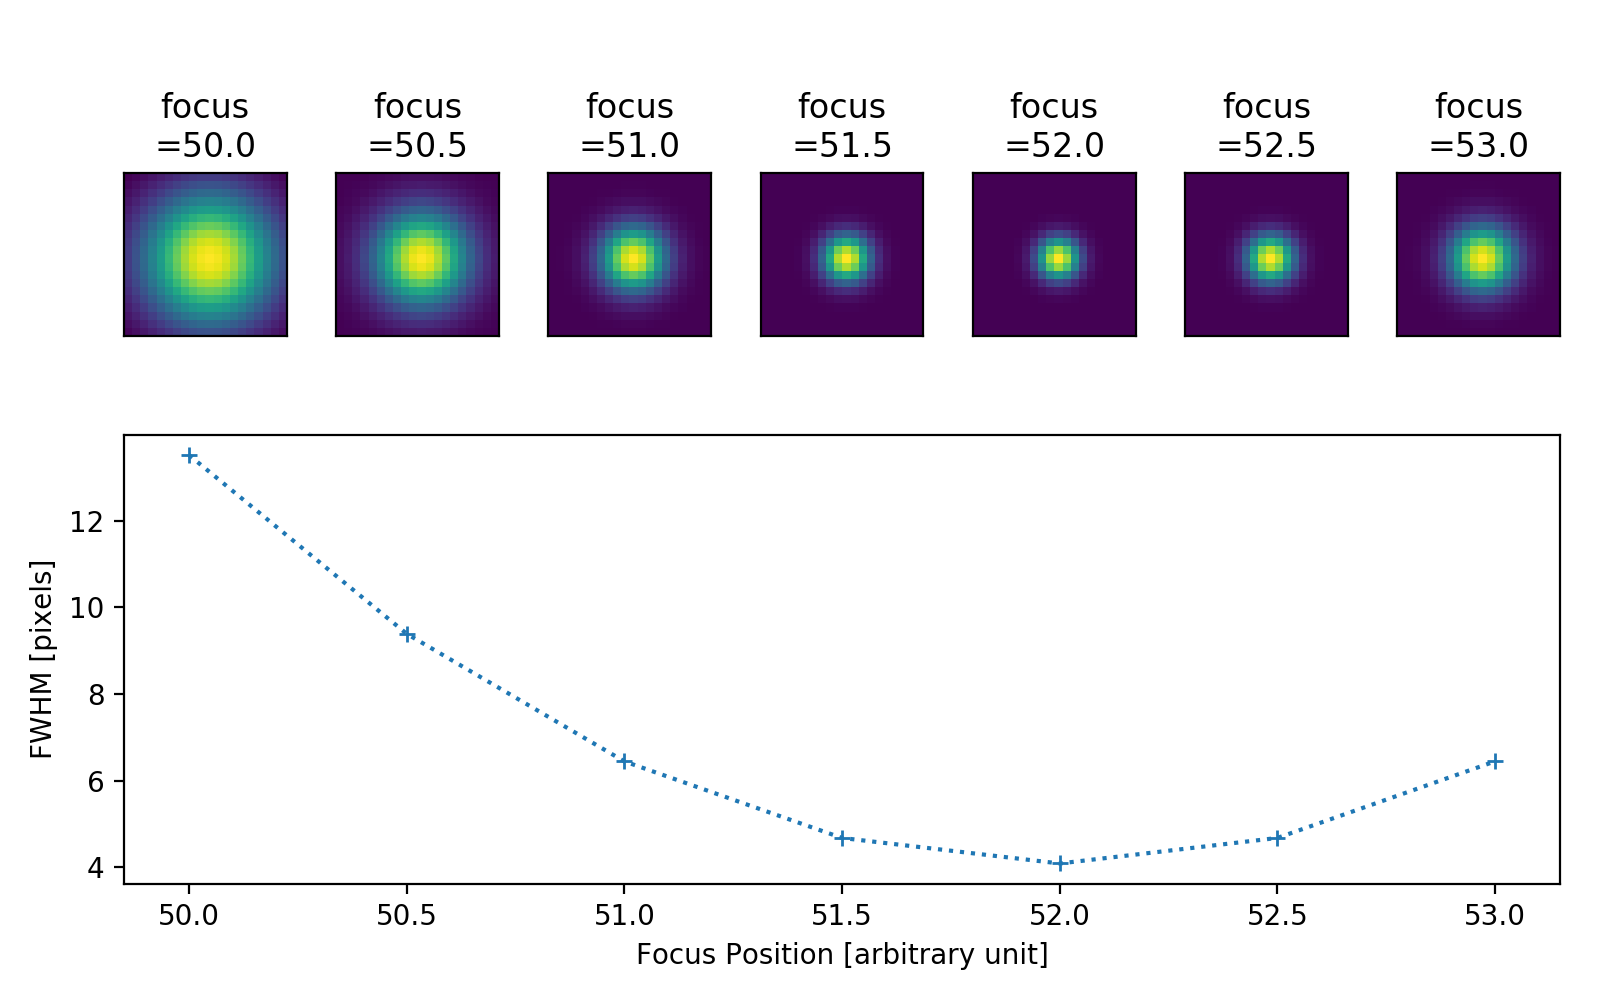
\includegraphics[width=0.7\linewidth]{figs/focusing}
  \caption{Finding focal position. While tuning the focal position value (x-axis), check the FWHM of the stellar profile. In this fake simulation, it is found that the focal position of 52.0 is \textit{the} focal position with FWHM $ \sim 4 $ pixels. Multiplying with the pixel scale will give the FWHM in angular units (e.g., if the pixel scale is $ \SI{0.8}{arcsec/pixel} $, FWHM after the focusing is $ \SI{4}{pixel} \times \SI{0.8}{arcsec/pixel} = \SI{3.2}{arcsec} $)}
\label{fig:focusing}
\end{figure}


Our goal in observation is to ``gather all the photons from the target''. For a faint source, you have to tune the focal position very accurately, so that the signal from the source gathers to as small number of pixels as possible. Otherwise, the signal will be buried in sky values or other noise sources (dark current or readnoise) and our goal may not be achieved. The non-circular PSFs for high-quality data shares this same philosophy: the ``sprays'' of PSF should be analyzed. But for a very bright source, you may even intentionally defocus before the exposure. This is because we can avoid saturation and blooming from the central pixels while the signal is so strong that the noise is overwhelmed by the source signal. Then our goal is achieved even if we forget about the accurate focal position or accurate PSF.


\section{Centroid}
Even though we know the accurate PSF, we cannot use it for photometry if we cannot determine the center or the origin. There are various ways to determine this ``origin'', but the most widely used one is centroiding (center of mass). 

%but most of them have one or more of the following drawbacks: (1) no analytic solution but numerical calculation needed, (2) computationally heavy, (3) formulated only by empirically. One of the useful analytical centroiding is given here.

Let $ I_i $ for $ i = 1, 2, \cdots , N $ means the $ i $-th pixel with $ (x, y) = (x_i, y_i) $ of the original $ N_x \times N_y $ 2-D pixel array so that $ N = N_x N_y $. Say we set a threshold $ I_0 $ (e.g., background value, signal-to-noise ratio of 3, etc). Then change $ I_i = 0 $ if $ I_i < I_0 $. For $ \xi = x $ or $ y $, the centroid is by definition
\begin{equation} \label{eq: centroid}
  \xi_c = \frac{\sum_i I_i \xi_i}{\sum_i I_i} ~.
\end{equation}
The uncertainty of this is, considering $ \xi_i $'s are fixed with no uncertainty,
\begin{equation}
  \qty (\Delta \xi_c)^2
    = \qty(\pdv{\xi_c}{I_1})^2 \qty(\Delta I_1)^2 
      + \cdots + \qty(\pdv{\xi_c}{I_N})^2 \qty(\Delta I_N)^2 ~.
\end{equation}
But
\begin{equation}
  \pdv{\xi_c}{I_k} 
    = \pdv{I_k} \qty( \frac{I_1 \xi_1 + \cdots + I_N \xi_N}{I_1 + \cdots + I_N} )
    = \frac{\xi_k}{\sum_i I_i} - \xi_c ~,
\end{equation}
so
\begin{equation}
  \qty (\Delta \xi_c)^2
  = \sum_k \qty(\frac{\xi_k}{\sum_i I_i} - \xi_c)^2 \qty(\Delta I_k)^2
  = \frac{\sum_k (\xi_i - \xi_c)^2 \qty(\Delta I_k)^2}{\sum_i I_i} ~.
\end{equation}
Pixels near the object are likely to have high pixel values, so we approximate the uncertainty $ \Delta I_i $ is just the Poisson noise of the pixel value (which is source $ + $ sky $ + $ read noise), i.e., m \cref{eq: Pois mean std}, $ \Delta I_i = \sqrt{I_i} $. Then expanding the square and using the definition of $ \xi_c $, we get
\begin{equation} \label{eq: centroid err}
  \Delta \xi_c 
  = \sqrt{\frac{\sum_k (\xi_i - \xi_c)^2 I_k }{\sum_i I_i} }
  = \sqrt{\frac{s_c^2}{\sum_i I_i}}
\end{equation}
where
\begin{equation}
  s_c^2 = \frac{\sum_k \xi_k^2 I_k}{\sum_i I_i} - \xi_c^2 ~.
\end{equation}


There are some other techniques which involves Gaussian fitting: marginalize the image onto the $ x $- and $ y $-axes, and do the 1-D Gaussian fitting to each of them. Also the sigma-clipping inside the centroiding box (cbox) can be used (e.g., Ma+ 2009, Opt.Exp., 17, 8525).

\section{Aperture Sum}
We need first to find the total flux inside the aperture. The sky subtraction will be done later. Consider a very simple case in \cref{fig:photapex01}: The centroid is calculated following \cref{eq: centroid}, and it is trivial that the centroid is at the center of the shown image. If we put circular aperture of radius 1 pixel (middle panel), the pixel contribution from the pixel with value 10 (right panel) is
\begin{equation}
  \mathrm{pixel~value} \times \frac{\mathrm{area~in~aperture}}{\mathrm{total~area}}
  = 10 \times \frac{\pi / 4}{1}
  = 7.854 ~.
\end{equation}
Doing the same calculation for all the 4 pixels inside the aperture, you will get $ N_\mathrm{apsum} = 47.12 $, where apsum means the ``aperture sum''. 

\begin{figure} [ht!]
\centering
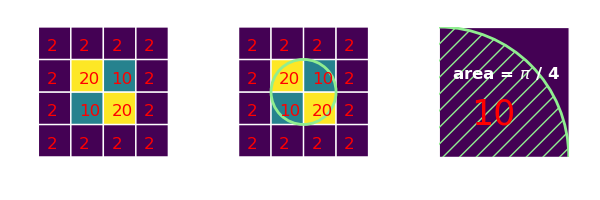
\includegraphics[width=0.7\linewidth]{figs/phot_ap_ex01}
\caption{Left: An example pixel values near the source. Middle: An aperture of radius 1 pixel shown as green circle. Right: A zoom in of one pixel with pixel value 10.}
\label{fig:photapex01}
\end{figure}

One thing to note is the uncertainty in position. In this 4 by 4 pixel example, $ \sum_i I_i = 84 $ and $ \xi_c = (x_c, y_c) = (1.5, 1.5) $ under the 0-indexing. For $ \Delta x_c $, we consider only the $ x $-coordinate for \cref{eq: centroid err} caluclation. Note that in that case, $ \sum_k (x_k^2 I_k) $ for all the $ \num{4 x 4} = 16 $ pixels is nothing but $ \sum_{k=1}^{4} (x_k^2 I'_k) $ where $ I' = [8,\, 34,\, 34,\, 8] $ is the marginalized intensity along the $ x $ direction from \cref{fig:photapex01}. Then $ \Delta x_c = 0^2 \times 8 + 1^2 \times 34 + 2^2 \times 34 + 3^2 \times 8 = 242 $. This must be the same for the $ y $-axis, and thus $ s_c^2 = 242 / 84 - 1.5^2 = 0.63 $, so $ \Delta x_c = \Delta y_c = \sqrt{0.63 / 84} = 0.087 $ pixel.

Here, I did not touch the topics such as (1) how to select the aperture radius, $ r_\mathrm{ap} $ and (2) in reality, we need to fit some function to the radial profile, but which function should we use? These will be dealt in the next chapter.

Since this aperture sum includes not only the source but also the sky values (sky value is always non-zero for ground-based observations), we need to subtract the sky.


\section{Sky Estimation}
Estimation of the sky is one of the most trickest part in observational astronomy. There are two most widely used methods: annulus and 2D interpolation. I will first explain few formulae, and then explain these two methods.

\subsection{Simple Parametric Sky Estimation}
There have been some parametric methods to estimate correct sky value. The most widely used ones include the ``MMM'' relation, or the ``mean-median-mode'' relation, and regard the mode (most frequent value) as the constant sky value. This has been used by virtually all astronomical softwares, including IRAF, IDL, SExtractor, and python packages. It is the simplest and does not require much computational speed, while gives reasonable results in many cases.

Why mode? The mission in determining the \textit{constant} sky value is to find a \textit{robust}, i.e., trustful constant value. Average (mean) is very vulnerable to few outliers even though we did sigma-clipping, and the median is less robust than mode, because if faint object with $ S/N $ ratio $ \sim 1 $ is in the sky region, the median can also be overestimate the sky. Thus, mode is the most widely used simple statistic for sky estimation.

The determination of the modal value is very difficult, because the it is not simple to define it for the \textit{sampled data}. If the distribution is not a mathematically continuous one, i.e., if it is discrete as we always encounter after sampling process, the mode is the largest value when we draw a \textit{histogram}. The histograms are basically sensitive to the subjective selection of bins, and you can change the modal value to an unexpected value depending on the bin you choose (see \cref{fig:phottestsky01}). %It gets very complicated because the pre-processed image can have real number values, not integers. Hence, the histogram may look like a comb with only 1 count at each comb, if the bins are set to be infinitesimally small. 

\begin{figure}[ht!]
\centering
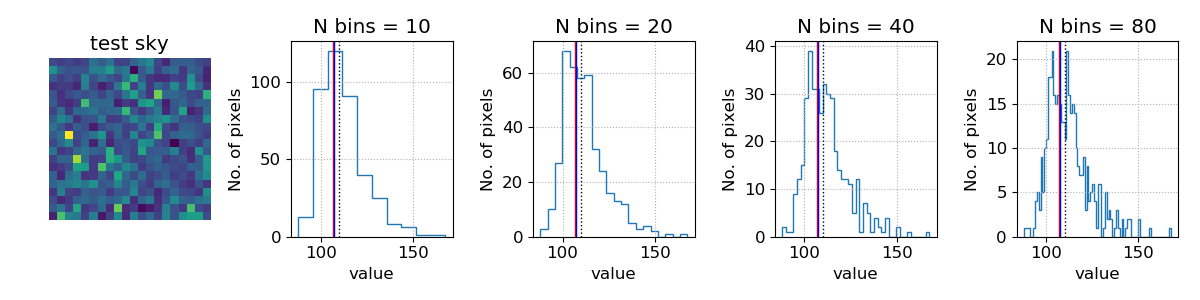
\includegraphics[width=\linewidth]{figs/phot_testsky01}
\caption{Left: A fake sky of 20 by 20 pixels generated by $ 100 + \mathcal{N}(0, 5^2) + 5 \chi^2_2 + 3 \mathcal{U}(0, 1) $ (normal distribution, chi-squared distribution, and uniform distribution, respectively). Others: The histogram of the pixel values with different bin numbers with fixed bin width. The black dotted lines is the median, and the red and blue solid lines are the mode estimation from \cref{eq: mmm 3 2,eq: mmm sex}, respectively (almost indistinguishable). As can be seen, the mode value does not lie at the same position, and it even become bimodal when the number of bins is 80.}
\label{fig:phottestsky01}
\end{figure}

Since 1800s, people empirically knew that the mode has the following relationship which holds for a moderetely asymmetric distribution:
\begin{equation}\label{eq: mmm 3 2}
  \mathrm{mode} \approx 3 \times \mathrm{median} - 2 \times \mathrm{mean} ~,
\end{equation}
or equivalently, \textit{the distance between the mode and median is two-thirds of that between mode and mean}. DoodsonAT (1917, Biometrika Trust, 11, 425) first gave mathematical proof of it using some mathematical tricks including Laplace's and De Morgan's (1836), and it is recognized by many statisticians including KendallMG (1943; or the second edition of it in 1945, The Advanced Theory of Statistics 2e, Vol 1, p.35). People now refer to more recent references like KendallMG+StuartK (1977, The Advanced Theory of Statistics, Vol. 1. Charles Griffin \& Co., London).

SExtractor (BertinE+ArnoutsS, 1996, A\&AS, 117, 393) uses a variant of this:
\begin{equation}\label{eq: mmm sex}
  \mathrm{mode} \approx 2.5 \times \mathrm{median} - 1.5 \times \mathrm{mean} ~.
\end{equation}
There is no clear reason provided in the original paper nor the SEx user manual, but it is just descibed that it was found to be more accurate when they tested. The estimation process works like this: Get the mean, median, and sample standard deviation (mean, med, std, respectively) from the sky pixel values after sigma-clipping. If $ \frac{\mathrm{mean} - \mathrm{med}}{\mathrm{std}} > 0.3 $, use $ \mathrm{mode} \approx \mathrm{med} $\footnote{Although the publication and SEx manual says they use mean if $ \frac{\mathrm{mean} - \mathrm{med}}{\mathrm{std}} > 0.3 $, but the SEx software actually returns med, not mean (described in photutils v0.6, Background Estimation (photutils.background))}. Otherwise, use \cref{eq: mmm sex}. 

IDL MMM uses \cref{eq: mmm 3 2}. IRAF also uses \cref{eq: mmm 3 2} internally, but it gives the mean value if $ \mathrm{mean} < \mathrm{med} $. In astropy-related packages (e.g., \texttt{photutils}), it is the user's choice. In all cases, you can set the sigma-clipping factors, e.g., $ a $ such that data outside $ \mathrm{med} \pm a \times \mathrm{std} $ can be rejected, and $ n $, the maximum iterations this process should be done until no more data are rejected. Whether to use $ \mathrm{med} \pm a \times \mathrm{std} $ or $ \mathrm{mean} \pm a \times \mathrm{std} $, whether to give asymmetric $ a $ values (upper and lower sigma-clipping), etc are up to the user.

I recommend to follow what SEx does, with sigma-clipping of $ a \sim 3 $ and $ n \ge 5 $, because that became a virtual standard in parametric sky estimation.


\subsection{Other Ways for Sky Estimation}
As can be seen from \cref{fig:phottestsky01}, the sky histogram is mostly skewed towards right. Because of this, BijaouiA (1980, A\&A, 84, 81) first introduced to fit the sky histogram with Gaussian multiplied by Laplace:
\begin{equation}
  p(I) = \frac{e^{\sigma^2 / 2 a^2}}{a} e^{-(I - s) / a} \mathrm{erf}_c \qty(\frac{\sigma}{a} - \frac{I - s}{\sigma})
\end{equation}
where
\begin{equation} 
  \mathrm{erf}_c(x) := \frac{1}{\sqrt{2\pi}} \int_x^{+\infty} e^{-t^2/2} dt ~.
\end{equation}
IrwinMJ (1985, MNRAS, 214, 575) argued that this method for modal estimation (Bayesian maximum likelihood is used) is better compared to mean, median, and Gaussian fitting. But because of the complexity of the calculation, Irwin used simpler method, i.e., get the smoothed histogram near the estimated mode and fit a Gaussian. BeardSM+ (1990, MNRAS, 247, 311) used slightly different method: smooth the (sky pixel) frequency histogram with moving box filter, find the mode estimate with it, sample the pixels nearby it which has pixel values larger than half of it. Then it does a cubic polynomial fit to the unsmoothed original histogram and finds the peak from this polynomial as the mode estimate.

For more, you may refer to Appendix A of AkhlaghiM and IchikawaT (2015, ApJS, 220, 1) and section 3.1 of MasiasM+ (2012, MNRAS, 422, 1674). 


\subsection{Annulus Sky}
The simplest way is to use circular annulus. This method assumes the sky is nearly constant near the terget of interest, PSF is circular, and there is no nearby celestial object. Under these simplifying assumptions, the sky must be azimuthally symmetric and a function of radius centered on the centroid of the target. If we set the inner and outer radii $ r_\mathrm{in} $ and $ r_\mathrm{out} $ much larger than the seeing disc size to define the circular annulus, the pixel values within that annulus are now the ``sample'' of sky values, and should not have clear tendency along the radial and azimuthal direction. \cref{fig:photapex02} shows the result of centroiding and sky estimation. 

\begin{figure} [ht!]
\centering
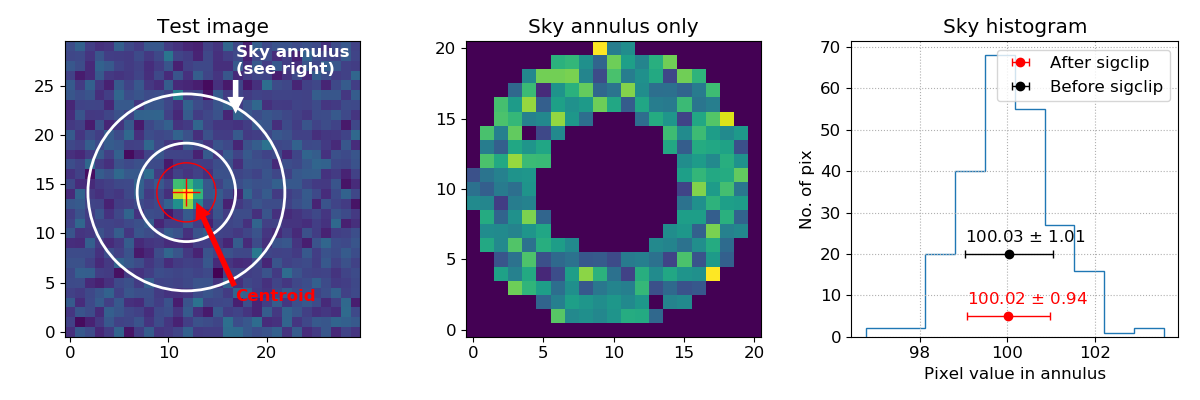
\includegraphics[width=\linewidth]{figs/phot_ap_ex02}
\caption{Left: The test image. Centroid is determined by \cref{eq: centroid} and annulus is defined as $ r_\mathrm{in} = 5 $ and $ r_\mathrm{out} = 10 $ pixels, respectively. Middle: Plotting the sky annulus region only, to just visualize the random fluctuations in the sky region. Clearly, there is no radial trend and it seems quite symmetric along the azimuth. Right: The histogram of the sky pixel values in the annulus. The red/black markers are the median and sample standard deviation of the sky values after and before sigma-clipping, respectively. The sigma clip was done with 3-sigma 50-iterations.}
\label{fig:photapex02}
\end{figure}

Consider we obtained the sky value $ m_\mathrm{sky} $ somehow, e.g., median of sky, \cref{eq: mmm sex} after sigma-clipping, etc. There can be many ways to estimate the uncertainties of this $ m_\mathrm{sky} $. Let me call this $ \Delta m_\mathrm{sky} $. The fluctuation of sky value can critically affect the final result of the photometry. But once a robust way to estimate the sky is set and if the target is bright enough, the uncertainty due to the sky value is not so large. Thus, people do not care too much about the accurate pdf of the $ m_\mathrm{sky} $ value. The most widely used way is to use the practical CLT (Thm \ref{thm: practical clt}) to $ m_\mathrm{sky} $, treating as if it is the mean of the sky samples (although we almost never use the mean for $ m_\mathrm{sky} $). Then
\begin{equation}\label{eq: err m_sky}
  \Delta m_\mathrm{sky} = \frac{s_\mathrm{sky}}{\sqrt{n_\mathrm{sky}}} ~.
\end{equation}
Here, $ s_\mathrm{sky} $ and $ n_\mathrm{sky} $ are the sample standard deviation and the number of the sky pixels survived after the sigma-clipping, respectively. So we are assuming here that the mode has similar uncertainty as the mean.




\subsection{Source Extractor Sky}
We will not cover Source Extractor (SE or SEx or SExtractor) deeply. But simply put, it works like the description below. Say we have the image of 1000 by 1000 pixel.

\begin{enumerate}
\item \textbf{Meshing}: Chop the image by given box size. For example, if you set the box size as $ (50, 25) $, 20 by 40 (in total 800) ``pads'' or ``meshes'' will be made. Each pad will of course have 50 by 25 (in total 1250) pixels.
\item \textbf{Filtering}: Determine the size of the median filter. If the size is $ (3, 3) $, for instance, a 3 by 3 median filter will be used to reduce sharp noised pixels in each pad (similar to Gaussian convolution). The filter size should be determined as a function of seeing disc size. 
\item \textbf{Rejecting Meshes}: In this median-filtered pad, the sigma-clipping is done. If too many pixels inside a pad is rejected, that pad is rejected for the next background estimation step. Such a threshold, say exclusion percentile, must be given by the user. For example, if that percentile is 10 \%, any of the 800 mesh which rejected more than 10 \% of its pixels from sigma-clipping (10 \% out of 1250 pixels, i.e., 125 pixels) will be regarded as ``bad region'' for the sky estimation.
\item \textbf{Sky at each Mesh} (bottom middle panel of \cref{fig:sexbkg01}): Now come back to the original un-filtered meshes. From the pixel values, estimate the sky value and its uncertainty following \cref{eq: mmm sex} and the description below the equation. For the meshes which are flagged as ``bad'' from previous step are not used for this process. As a result, you will have 20 by 40 array of sky values, while some elements may be empty or NaN, if some meshes are flagged ad ``bad''.
\item \textbf{Interpolation} (top middle panel of \cref{fig:sexbkg01}): From the estimated single sky value at each mesh, i.e., the 20 by 40 array, we do interpolation to estimate the sky at all the 1000 by 1000 pixels. The estimation uncertainties should also be calculated for each pixel.
\end{enumerate}

\begin{figure}[ht!]
\centering
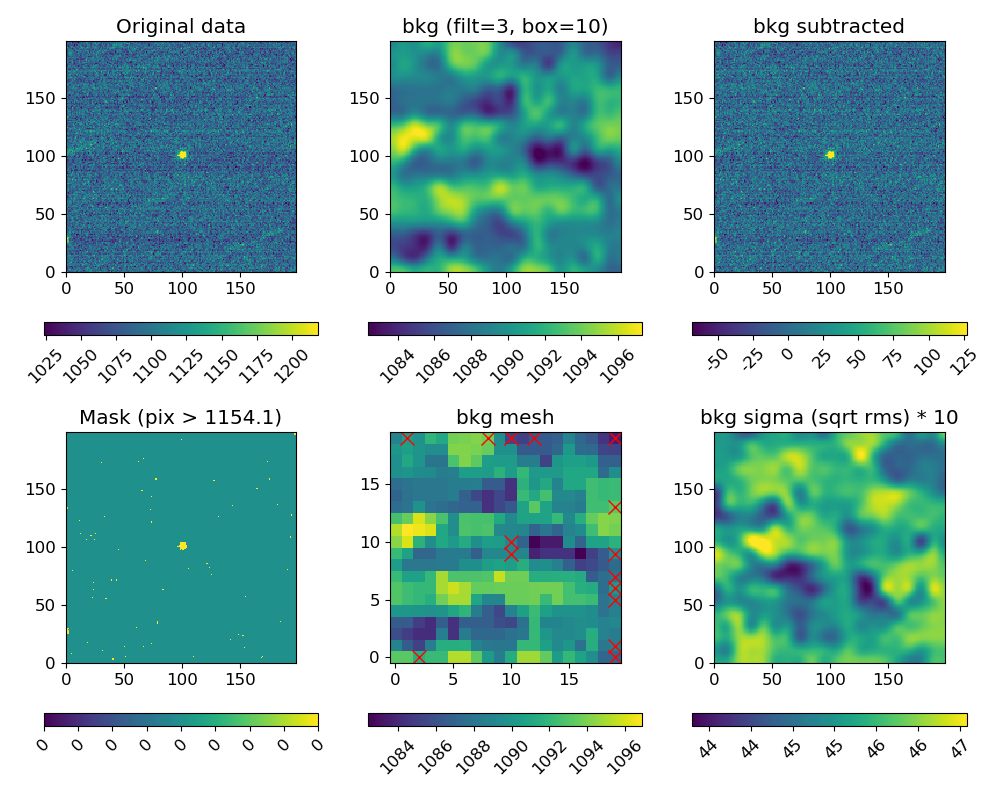
\includegraphics[width=\linewidth]{figs/sex_bkg_01}
\caption{Example of the SExtractor background estimation usage. The original data is the targeto-centric combined image from 13 KMTNet images from SAAO observatory. The pixels with value 1154.1, which is the $ \mathrm{med} + 3\mathrm{std} $ after the sigma-clipping (3-sigma, 5-iter clipping) are masked because those can be stars (bottom left). The background meshes with the estimated sky values (\cref{eq: mmm sex}) are shown in bottom center, and the interpolated one is given in top middle. Note that the sky level changes at maximum around 12 ADU out of the pixel value 1000+. Normally this should be smaller like 5 ADU or 2 ADU within this small region (200 by 200 pixel). The background sigma shown in bottom right is around 4 ADU (note the figure is 10 times the sigma), but many times the sky sigma is smaller than this.}
\label{fig:sexbkg01}
\end{figure}

After the sky subtraction, I plotted the Box plot of the image with x-axis 70 to 90 and y-axis 50 to 150 (python indexing) in \cref{fig:sexbkg02skyhist}.

\begin{figure}[ht!]
\centering
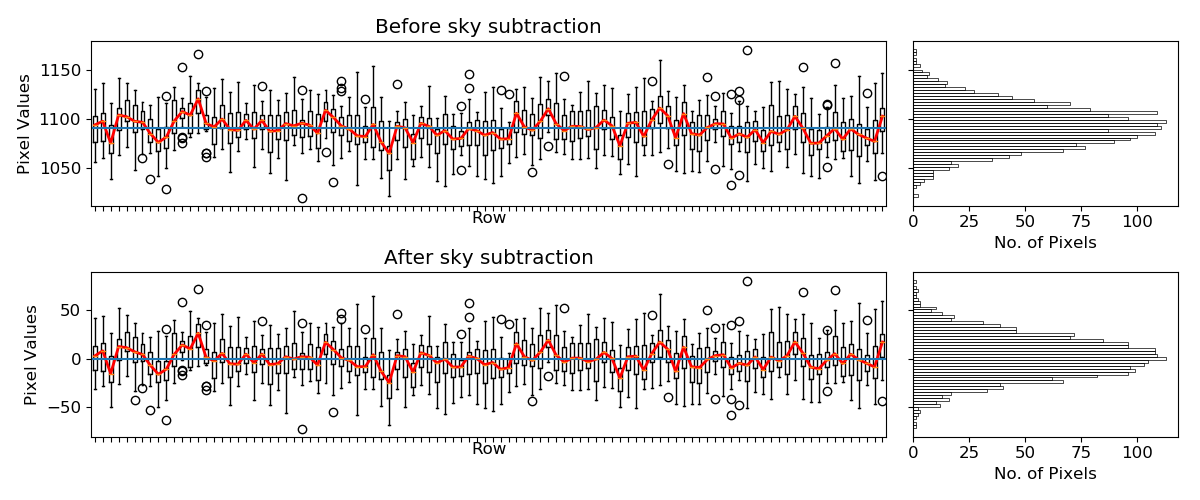
\includegraphics[width=\linewidth]{figs/sex_bkg_02_skyhist}
\caption{The Box plot and pixel value histogram of before/after the sky subtraction, of a region defined by \texttt{data[50:150, 70:90]} (python indexing). The horizontal axes of Box plots correspond to the ``row'' or the y index. Blue horizontal lines are the median of all the pixels in that region, and red solid lines are the medians }
\label{fig:sexbkg02skyhist}
\end{figure}

As can be noticed, SEx background estimation\footnote{We tend to call ``background'' rather than ``sky'' when we are dealing with SExtractor.}, unlike the annulus sky estimation technique, is estimating the sky values at all the pixels, not for each source. Thus, it takes much longer time. Also you can see that lots of parameters (rejection percentile, box size, filter size, interpolation method and related parameters, etc) should be set for SEx to work! In some cases, astronomers run SExtractor again and again to do get expected results, and find best combination of such parameters. But these parameters of course depend on the instruments, sky conditions, etc, so if the results are suspicious, some fine tuning must be made or you have to find different ways to do photometry than SExtractor.





\end{document}